\everymath{\displaystyle}
\documentclass{beamer}
% \documentclass[handout]{beamer}

%\usepackage[pdftex]{color,graphicx}
\usepackage{amsmath,amssymb,amsfonts}

\mode<presentation>
{
  % \usetheme{Darmstadt}
  % \usetheme[hideothersubsections]{Hannover}
  % \usetheme[hideothersubsections]{Goettingen}
  \usetheme[hideothersubsections, right]{Berkeley}

  \usecolortheme{seahorse}
  % \usecolortheme{dolphin}
  \usecolortheme{rose}
  % \usecolortheme{orchid}

  \useinnertheme[shadow]{rounded}

  \setbeamercovered{transparent}
  % or whatever (possibly just delete it)
}

\mode<handout>{
  \setbeamercolor{background canvas}{bg=black!5}
  \usepackage{pgfpages}
  \pgfpagesuselayout{4 on 1}[a4paper,border shrink=5mm, landscape]
}

\usepackage[brazilian]{babel}
% or whatever

% \usepackage[latin1]{inputenc}
\usepackage[utf8]{inputenc}
% or whatever

\usepackage{times}
%\usepackage[T1]{fontenc}
% Or whatever. Note that the encoding and the font should match. If T1
% does not look nice, try deleting the line with the fontenc.


\title%[] % (optional, use only with long paper titles)
{Etapas da Pesquisa}

\subtitle
{Planejamento, Buscas e Perdas} % (optional)

\author%[] % (optional, use only with lots of authors)
{Felipe Figueiredo}% \and S.~Another\inst{2}}
% - Use the \inst{?} command only if the authors have different
%   affiliation.

\institute[] % (optional, but mostly needed)
{
}
  % \inst{1}%
  % Department of Computer Science\\
  % University of Somewhere
  % \and
  % \inst{2}%
  % Department of Theoretical Philosophy\\
  % University of Elsewhere}
% - Use the \inst command only if there are several affiliations.
% - Keep it simple, no one is interested in your street address.

\date%[] % (optional)
{}

% \subject{Talks}
% This is only inserted into the PDF information catalog. Can be left
% out. 



% If you have a file called "university-logo-filename.xxx", where xxx
% is a graphic format that can be processed by latex or pdflatex,
% resp., then you can add a logo as follows:

\pgfdeclareimage[height=1.6cm]{university-logo}{../logo}
\logo{\pgfuseimage{university-logo}}



% Delete this, if you do not want the table of contents to pop up at
% the beginning of each subsection:
\AtBeginSubsection[]
%\AtBeginSection[]
{
  \begin{frame}<beamer>{Sumário}
    \tableofcontents[currentsection,currentsubsection]
  \end{frame}
}


% If you wish to uncover everything in a step-wise fashion, uncomment
% the following command: 

\beamerdefaultoverlayspecification{<+->}


\begin{document}

\begin{frame}
  \titlepage
\end{frame}

\begin{frame}{Sumário}
  \tableofcontents
  % You might wish to add the option [pausesections]
\end{frame}


%% Template
% \section{}

% \subsection{}

% \begin{frame}{}
%   \begin{itemize}
%   \item 
%   \end{itemize}
% \end{frame}

% \begin{frame}
%   \begin{columns}
%     \begin{column}{5cm}
%     \end{column}
%     \begin{column}{5cm}
%     \end{column}
%   \end{columns}
% \end{frame}

% \begin{frame}{}
%   \includegraphics[height=0.4\textheight]{file1}
%   \includegraphics[height=0.4\textheight]{file2}
%   \includegraphics[height=0.4\textheight]{file3}
%   \begin{figure}
%     \caption{}
%   \end{figure}
% \end{frame}

% \begin{frame}{}
%   \begin{definition}
%   \end{definition}
%   \begin{example}
%   \end{example}
%   \begin{block}{Exercício}
%   \end{block}
% \end{frame}

\section{Planejamento}

\subsection{Preparação da Pesquisa}

\subsection{Fases da Pesquisa}

\subsection{Execução da Pesquisa}

\subsection{Relatório da Pesquisa}



\section{Buscas}

\subsection{Google Scholar}


\section{Fracassos}

\subsection{Fracassos?}

\begin{frame}{Rejeição}
  \begin{itemize}
  \item Diversos motivos podem levar à rejeição do texto
  \item Revisão por pares = escrutínio de todos os detalhes
  \item Análise da metodologia e argumentação
  \item Detecção de possíveis fraudes
  \end{itemize}
\end{frame}

\begin{frame}{O {\em peer review} não é perfeito}
  \begin{itemize}
  \item Somos todos humanos:
    \begin{itemize}
    \item rejeição por motivos pessoais
    \item ideologia
    \end{itemize}
  \item Falha na revisão
  \item Aceitação de estudos {\em fake}
  \item Rejeição de estudos {\em válidos}
  \end{itemize}
\end{frame}

\begin{frame}{Preconceito}
  Artigo rejeitado pois as autoras eram mulheres, não havia nenhum
  homem no grupo
    \begin{block}{O revisor}
      \ldots find one or two male biologists to work with (or at least
      obtain internal peer review from, but better yet as active
      co-authors), in order to serve as a possible check against
      interpretations that may sometimes be drifting too far away from
      empirical evidence into ideologically based assumptions.
    \end{block}

\url{http://retractionwatch.com/2015/04/29/its-a-mans-world-for-one-peer-reviewer-at-least/}
\end{frame}

\begin{frame}{Preconceito}
  Artigo rejeitado pois as autoras eram mulheres, não havia nenhum
  homem no grupo
    \begin{block}{A revista}
      PLOS regrets the tone, spirit and content of this particular
      review. We take peer review seriously and are diligently and
      expeditiously looking into this matter. The appeal is in
      process. PLOS allows Academic Editors autonomy in how they
      handle manuscripts, but we always follow up if concerns are
      raised at any stage of the process. Our appeals policy also
      means that any complaints of the review process can be fully
      addressed and the author given opportunity to have their paper
      re-reviewed.
    \end{block}

\url{http://retractionwatch.com/2015/04/29/its-a-mans-world-for-one-peer-reviewer-at-least/}
\end{frame}

\begin{frame}{Ou seja...}
  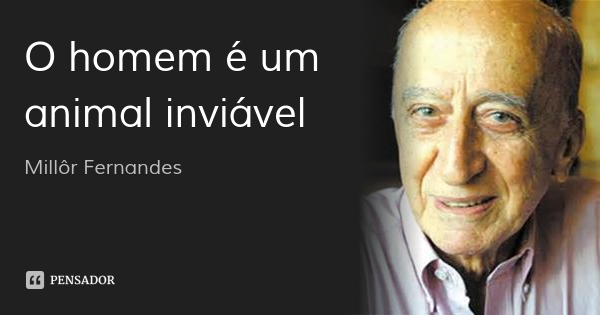
\includegraphics[width=\textwidth]{millor}
\end{frame}

\end{document}
